\documentclass[10pt,twocolumn,letterpaper]{article}
\usepackage[margin=0.72in]{geometry}
\usepackage[T1]{fontenc}
\usepackage[utf8]{inputenc}
\usepackage{amsmath,amssymb,booktabs,graphicx}
\usepackage[hidelinks]{hyperref}
\setlength{\columnsep}{0.24in}
\setlength{\parskip}{2pt}
\raggedbottom
\setlength{\emergencystretch}{1.5em}
\graphicspath{{figures_003/}{paper/figures_003/}}
\newcommand{\NA}{\textnormal{NA}}
\newcommand{\archive}[1]{\path{#1}}
\Urlmuskip=0mu plus 1mu
\title{From Verification Savings to Repair Limits:\\A Retrospective Methodological Evaluation of ProbeFlow}
\author{Gyeongtae Im\\Independent Researcher\\\texttt{gyeongtaeim.research@gmail.com}}
\date{November 23, 2026\\\small Research draft for methodological review; not a claim of publication readiness}

\begin{document}
\maketitle
\begin{abstract}
When an automated research program changes direction after a negative result, the new question should follow from an identified limitation rather than from a more favorable metric. We examine six such changes in ProbeFlow, using archived protocols, implementations, and result receipts from November 16--20, 2026. Costed verification of 880 public code-candidate verdicts produced conditional savings in virtual units but tied a strong fixed-batch Bayesian baseline. Controlled timing on 144 synthetic batches did not establish general speedup. A tool-query compiler reduced additional reads from 46 to 3 on 23 action prefixes, while an explicit classical decision procedure achieved the same result. Actual local-model policy generation and repair produced no completely correct rule in four authored families; a subsequent diagnostic showed that the restricted repair language could fully repair at most one family. Finally, an external security-log study evaluated 65 accessible FoRGe tasks. A frozen 17-task confirmation yielded description-prior macro F1 of 0.537 but pooled F1 of only 0.075, with 2,409 false positives. A post-hoc counterexample follow-up on those same tasks reached pooled F1 of 0.598 versus 0.260 for a shared-pool length selector, after 4,390 development-label comparisons returned 22 labels. This is exploratory evidence, not fresh confirmation. We give explicit cost accounting, reconstruct the implemented selectors, and distinguish information, representation, selection, and evaluation limits. The resulting contribution is a bounded methodological case study, not a new synthesis algorithm, efficiency guarantee, or frontier-model comparison.
\end{abstract}

\section{Introduction}
An agent that checks, repairs, or regenerates an artifact makes several decisions that are easy to conflate. It decides what information to acquire, whether that information can distinguish the relevant states, whether its repair language can express a correct artifact, and which feasible candidate to select. A reduction in checks answers only one of these questions. A more accurate candidate may still be expensive to obtain; a cheap rule may create too many false alarms; and perfect consistency with a few counterexamples may leave an omitted input unrepresented.

ProbeFlow began with questions about repeated attempts, transitions, and verification. This paper reconstructs a narrower, documented sequence in which stronger controls repeatedly changed the question. We examine six archived studies, ending with a security-log experiment on data produced by a separate research team. These studies have different units, assumptions, and evaluators. We do not combine their results into a single performance curve. Instead, we ask which observation justified each change of direction, which part of the previous claim survived, and which comparison remained missing.

The final empirical question is deliberately modest: given a detection description, one positive seed, and a small number of development counterexamples, does a fixed lexical preference improve selection within a restricted regex class, and what does acquiring those counterexamples actually cost? Natural-language-guided synthesis, example consistency, and generate-and-repair are established ideas \cite{kushman2013,regel2020,sketchregex2020,transregex2021,opsynth2021}. FoRGe already studies the directly related single-seed security-log setting with an agentic feedback loop \cite{forge2026}. Accordingly, neither a lexical coverage objective nor repeated counterexamples establishes a new synthesis principle.

Our retrospective analysis has three concrete aims. First, it makes the units of evidence explicit: public verdict replays, controlled byte batches, tool action prefixes, authored policy families, and external log tasks. Second, it separates four failure mechanisms: inadequate observations, inadequate representation, poor selection within a class, and an evaluation that does not support the intended claim. Third, it shows how aggregate improvements and low returned-label counts can mislead when class imbalance, shared sources, full-pool label scans, and prior test exposure are omitted.

The endpoint is not a completed superiority result. The archived record supports conditional local improvements, several ties or negative results, and a post-hoc feedback signal worth testing elsewhere. It does not establish operational safety, total research-cost savings, independent-source generalization, superiority to strong natural-language-aware synthesis, or publication readiness.

\section{Study Scope and Evidence Discipline}
\label{sec:scope}
This is a retrospective methodological evaluation of existing local records, not a newly executed benchmark. The scientific experiments discussed below were archived before this manuscript. Manuscript preparation introduces no new target-model calls, policy experiments, or raw-corpus acquisition. The evidence map in Appendix~\ref{app:evidence} identifies the relevant protocols, code, and receipts. Local records are cited as unpublished artifacts, separately from external primary literature.

We use four evidence categories. An \emph{observed result} is a stored output of an executed local procedure. An \emph{author report} describes an external paper or artifact without implying reproduction. A \emph{diagnostic inference} follows from a fixed representation, code path, or stored evaluation. A \emph{future protocol} specifies an experiment not yet performed. Hash checks and independent recalculation can support artifact consistency; they do not authenticate a scientific interpretation or create human expert validation.

The evidence is not uniformly blind. The 880-verdict study had already exposed its overall pass/fail totals. The external-study leader had seen development results before the description-aware extension, although its separate implementer had not read the corpus, scores, or model responses when freezing the implementation. The 17 reserved tasks provided a subsequent frozen confirmation within that source. Their later counterexample analysis began after the confirmation results were known. We preserve this chronology rather than calling the whole sequence preregistered.

\begin{table*}[t]
\centering\small
\setlength{\tabcolsep}{4pt}
\begin{tabular}{p{0.13\textwidth}p{0.22\textwidth}p{0.28\textwidth}p{0.29\textwidth}}
\toprule
Study / question & Actual evidence unit & Observation that constrained the claim & Resulting methodological change\\
\midrule
P1: Pay to verify? & 880 fixed code candidates; 602 pass, 278 fail & Virtual-cost savings in some tariffs; 1,920 randomized trace comparisons tied guarded Bayes & Separate conditional decision value from algorithm superiority and measured runtime\\
P2: Is it faster? & 144 synthetic byte batches; 2,304 timed policy observations & Six audit alternatives lost in aggregate to a strong full-check reference & Measure actual overhead, quality allowances, caching, and parallel controls\\
P3: Which tool read? & 23 pending prefixes from 6 public tasks / 19 records & Additional reads 46/7/3; strong classical decision guard also 3 & Ask whether necessary semantics and adapters can be obtained, rather than claim a new query principle\\
P4: Repair or restart? & 4 authored policy families; 16,160 synthetic contexts & 12 actual generations; initial, continuation, restart each 0/4 exactly correct & Diagnose expressibility before increasing repair or query budgets\\
P5: Can this language repair? & Same 4 families; retrospective finite-state analysis & Constant-subtree repair ceiling 1/4; 3 families omit relevant inputs & Separate information acquisition from missing representation\\
P6: Does it transfer? & 65 accessible external tasks; 48 development, 17 reserved confirmation & Macro improvement coexisted with poor pooled detection; feedback follow-up reused the same 17 & Require new sources, stronger information-matched baselines, and complete feedback-cost accounting\\
\bottomrule
\end{tabular}
\caption{The six pivots concern different datasets and experimental units. Counts are not additive evidence for a common success rate. A repeated order, context, method branch, or log row does not become an independent research task.}
\label{tab:pivots}
\end{table*}

\section{A Common Decision and Cost Vocabulary}
\label{sec:formal}
Let $x$ denote a task state, $y(x)$ its operational reference label, and $h$ a decision rule. A procedure observes information $I$, may request additional observations $q_1,\ldots,q_k$, and returns an artifact, a decision, or an unresolved outcome. Its allowed hypothesis class $\mathcal H(I)$, query mechanism, and evaluator must be stated separately. A model may change $\mathcal H$ by writing a new expression; a fixed selector only chooses within its current class.

For an executed run, we distinguish the resource vector
\begin{equation}
\mathbf r=(n_{\rm req},t_{\rm tok},n_{\rm read},n_{\rm write},n_{\rm scan},n_{\rm ret},t_{\rm cpu},t_{\rm wall}),
\label{eq:resources}
\end{equation}
where $n_{\rm scan}$ counts labels compared while finding feedback and $n_{\rm ret}$ counts labels returned to a learner. These may differ substantially. An unknown component remains unknown. In particular, a timed-out accepted request with no usage report cannot be assigned zero tokens.

A scalar economic claim requires explicit tariffs and error consequences. One useful accounting identity is
\begin{align}
C_{\rm total}={}&C_{\rm prepare}+C_{\rm acquire}+C_{\rm generate}\nonumber\\
 &+C_{\rm enumerate}+C_{\rm verify}+C_{\rm fail}+C_{\rm decision}.
\label{eq:total}
\end{align}
The terms need not all be monetary. They should not be added across incompatible units without a declared conversion. Shared preparation, scans, and initial generations are charged once for an actual campaign. A hypothetical per-strategy composition can include its share explicitly, but summing those compositions would double-count common work. Zero additional target-model calls does not imply zero preparation, inference elsewhere in the research process, annotation, electricity, or total research cost.

For binary acceptance, the first study instantiated a narrower virtual objective. If $V$ is the verified set, $a_i\in\{\text{accept},\text{reject}\}$ is the decision for an unverified candidate, and $y_i=1$ means a stored pass verdict, then
\begin{align}
C_{\rm replay}={}&\sum_{i\in V}c(y_i)\nonumber\\
 &+L\sum_{i\notin V}\bigl[\mathbf1(a_i=\text{accept},y_i=0)\nonumber\\
 &\hspace{58pt}+\mathbf1(a_i=\text{reject},y_i=1)\bigr].
\label{eq:virtual}
\end{align}
This objective prices both erroneous acceptance and erroneous rejection. It is neither elapsed time nor a measured bill. The studies below progressively expose which components of a broader claim were absent from this restricted objective.

\section{Six Methodological Pivots}
\label{sec:pivots}
\subsection{P1: From repeated attempts to costed verification}
The archived verification experiment replays one fixed code candidate and one public verdict per problem \cite{pfpaid}. There are 880 unique problems, with 602 pass and 278 fail verdicts. Code strings were treated as data and were not executed anew. These are operational verdicts from the source evaluator, not a new proof of program semantics. Because there is only one candidate per problem, the data cannot evaluate switching among candidates or counterfactual sequences of code generation.

The replay compared a first admissible stopping policy, \texttt{FIRST\_GUARD}, with fixed-batch Bayesian policies, plug-in policies, and full verification, acceptance, or rejection. Public partitions were the full collection, three difficulty groups, and four code-length quartiles. Each problem belonged to exactly one group within a selected partition. Sixty-four fixed random orders and a separate chronological stress order changed observation order without creating new problems.

The tariffs used $L\in\{2,4,8,16,32\}$, pass-verification cost 1, and fail-verification cost 0.25 or 1. For the difficulty partition and $L=2$, mean virtual costs fell from 671.5 to 462.7734, and from 880 to 564.6563, respectively: savings of 31.08\% and 35.83\%. For the six conditions with $L=8,16,32$, the guarded procedure verified everything, producing zero savings. The price sensitivity is part of the result, not a nuisance to omit.

The guard allowed stopping only when both endpoints of a finite-population confidence interval gave a cost no worse than verifying the remaining items. Within each random order, error probability 0.05 was allocated across eight groups. This is a conditional, per-order statement under uniform random ordering; it is not a simultaneous 95\% guarantee over all 64 orders, and it does not cover the chronological stress order. Bayesian optimization applied to the specified Beta$(1,1)$ prior and fixed batch times, not to every possible query schedule.

Most consequentially, \texttt{FIRST\_GUARD} and same-partition guarded Bayes produced identical complete traces in all $3\times10\times64=1,920$ randomized comparisons, and in the 30 chronological comparisons. Thus the observed savings relative to full verification did not demonstrate a new algorithmic advantage. The next defensible question concerned actual acquisition overhead and measured time.

\subsection{P2: From virtual prices to measured timing}
The timing study used 144 controlled synthetic byte batches containing 18,432 artifacts and recorded 2,304 paired policy observations \cite{pfmeasured}. The measured operation was SHA-256 checking of in-memory bytes on one shared PC. There were no natural tasks, disk-I/O workloads, or target-model performance measurements in this experiment.

The full-verification reference included sequential and four-worker parallel implementations. Its selection depended on development calibration and artifact size. Six audit alternatives varied sampling, caching, confidence-based stopping, and parallelism. Their quality contracts permitted a defect allowance or bad-release risk that full verification did not require. A comparison therefore had to state both runtime and quality, rather than equate fewer checks with an identical guarantee.

Across the balanced condition grid, every audit alternative had greater aggregate policy time than the selected strong full-check reference, before adding calibration charges. A favorable condition illustrates the dependence on controls. With 262,144-byte artifacts, defect allowance $K=8$, and no defects, cached confidence-based sequential checking averaged 7.186 ms versus 13.067 ms for full sequential checking, but 4.953 ms for full parallel checking. A standard cached parallel audit averaged 2.556 ms in that condition. These conditional observations are not evidence for general speedup or for a new auditing algorithm.

The pivot was to ask where information acquisition has decision value under realistic overhead, rather than to treat virtual tariffs as an elapsed-time prediction. Calibration and process setup must be accounted for with their actual scope. Charging an entire timing acquisition to each alternative is an attribution sensitivity, not a second measured campaign or a fair independent deployment trial.

\subsection{P3: From checking more to reading only what changes an action}
A subsequent compiler experiment used 23 pending baggage-action prefixes from six public tasks and 19 records \cite{pfcompiler}. It reconstructed available information from tool responses preceding each pending action. The local adapter executed reviewed source methods, while subsequent dialogue, user simulation, and the official full evaluator were outside scope. No actual payment service was contacted.

On the original policy, reading the current reservation and profile for every action used 46 additional reads and 23 writes. An eager cache guard reduced reads to 7. A compiled decision guard reduced reads to 3 while preserving all 23 evaluated local completions. All reservations were already observed; 16 membership levels were observed and 7 were unknown. Four of the seven unknown cases had the same free-baggage decision at every allowed membership level. Three remaining prefixes required a profile read because membership changed the paid quantity.

An independently implemented classical decision guard enumerated the admissible hidden membership values and achieved the same three reads and evaluated outcomes. The proposed guard therefore established a resource improvement over full reads, but tied the strong information-matched comparison. The three necessary reads were also repeated prefixes for one user whose actual level was Gold. A post-hoc Gold-default diagnostic matched these stored outcomes without establishing a general zero-read guarantee. Sample regularity must not be mistaken for robust decision identifiability.

A separate authored price-conflict fixture changed a policy price from 50 to 40 while leaving the tool's charging coefficient at 50. The decision guard completed 21 free cases, deferred 2 conflicting paid cases, and used 2 reads, tying the classical guard. Avoiding a wrong charge is distinct from successfully delivering a paid service, and a smaller ledger increment is not money saved when actions were deferred.

Policy numbers and a narrow source-code coefficient were extracted mechanically. The calculation semantics, supported language, field mapping, and side-effect adapters were authored. This shifted the research question toward the cost and reliability of obtaining those meanings for new policies. It did not establish automatic general policy understanding or a new principle of partial observation.

\subsection{P4: From action guards to actual policy-generation failures}
The policy experiment formalized four subrules from two source policies: airline cancellation and compensation, and retail item exchange and return \cite{pfpolicy}. It fixed 128, 432, 15,552, and 48 authored synthetic contexts, respectively, totaling 16,160. These are four rule families, not 16,160 independent tasks. Authentication, ownership, target identity, and other prerequisites were fixed assumptions. The evaluator is an authored finite policy formalization, not a human certification of complete source-policy interpretation.

A local CPU-only \texttt{qwen3:14b} run made 12 actual generation calls: four initial, four continuation-repair, and four restart-repair calls. Continuation and restart received the same initial JSON and at most two identical development counterexamples; conversation roles and packaging differed. Restart did not physically reinitialize model weights. Outputs were data in a bounded DSL, not executed Python, SQL, or service commands.

The initial expressions were structurally valid for three families; the fourth was invalid and received no semantic accuracy. Neither the initial strategy nor either repair strategy produced a completely correct rule on any of the four families' test sets. Continuation and restart were structurally valid in all four, but each remained 0/4 exactly correct. Their principal matched-feedback comparison was therefore no gain in exact family completion, although partial error counts differed.

High aggregate accuracy hid consequential errors. For item exchange, the two repaired expressions were 99.6926\% accurate over 7,808 test contexts, yet allowed only 16 of 31 allowed cases and had 9 false allows and 15 false blocks. For compensation, both retained an unsupported restriction and blocked 10 of 26 allowed test cases. Return restart fit development examples but still falsely allowed one test case.

Provider-reported usage was 11,780 tokens: 3,387 initial, 4,166 continuation, and 4,227 restart. Strategy compositions including the common initial generation were 7,553 and 7,614 tokens; their sum is not the actual token expenditure because it double-counts the initial calls. Client times from this single execution also mix loading, cache, OS, and packaging effects, so they do not establish a general speed comparison.

An exploratory restricted repair replaced one subtree of a valid initial expression with true or false. Among 131 generated candidates, 87 were valid and 13 matched the supplied counterexamples. Selecting minimal behavioral change on unlabeled development contexts fully repaired compensation, while return still had an error; cancellation had no consistent candidate and exchange was structurally ineligible. This extra search evaluated candidates on unlabeled development inputs 1,942 times, so it was not information- and computation-identical to the two LLM arms. One repaired family motivated a representation diagnostic rather than a general success claim.

\subsection{P5: From additional counterexamples to representation limits}
The retrospective diagnostic grouped contexts by the fields visible to the initial expression \cite{pflimits}. Cancellation omitted \texttt{any\_flown}, exchange omitted \texttt{confirmed\_all\_items}, and return omitted \texttt{refund\_in\_profile}. These are fields on which the authored reference may depend. Replacing existing subtrees by constants cannot introduce a missing field.

The logic is elementary. Let $\phi(x)$ be the visible-field projection, and suppose every rule in a restricted class has form $h(x)=g(\phi(x))$. On a finite labeled collection, define $n_{z,0}$ and $n_{z,1}$ as the counts of the two labels in projection class $z$. Then every deterministic rule in that class makes at least
\begin{equation}
E_{\min}(\phi)=\sum_z\min(n_{z,0},n_{z,1})
\label{eq:lower}
\end{equation}
errors. Each group receives one prediction, so at least its minority label is wrong. In particular, two contexts with equal $\phi$ and different labels cannot both be classified correctly. This is a standard feature-equivalence diagnostic, not a new impossibility theorem about learning or program repair.

The full-context lower bounds were 58 errors for cancellation, 52 for any valid expression retaining exchange's missing-field restriction, and 1 for return. Exchange's invalid initial expression was not assigned those errors as a predictive score. Compensation had a correct candidate in the restricted repair class, yielding an exact-family ceiling of 1/4 for this repair language. Full-collection bounds can exceed the sum of partition-specific bounds because conflicting projection classes may straddle development and test. Computing these bounds used already-known full labels, including test labels; it is a retrospective explanation, not an inexpensive ex-ante predictor of repairability.

Additional simulated development queries compared fixed order, 16 random orders, generalized binary search, and exact optimal worst-case trees. In the closed version-space model, generalized binary search and the exact tree tied at worst-case depths of three for compensation and one for return. Identifying a remaining development behavior class did not fix return's missing-field error. Stored labels served as a simulated oracle; there was no newly measured human annotation cost.

An AI author subsequently wrote source-informed patches that passed all 16,160 existing contexts. Those four constructive examples show that an extended language can express the authored references. They are not four automatic discoveries on unknown policies, a 100\% automatic repair rate, a minimum-edit proof, or external expert validation. This boundary motivated external-source evaluation before further expanding an in-house grammar.

\subsection{P6: From authored policies to external security logs}
The external study fixed the FoRGe artifact at commit \texttt{d7e9175b8f718236369bcc1bfb1417ebbf68a7a4} \cite{pfexternal,forgeartifact2026}. Research Forge and the external FoRGe system are distinct. The external task is directly relevant: infer a detection regex from one positive log and an optional description, with feedback from log data \cite{forge2026}.

The upstream artifact declares 66 tasks and 19,428 log rows. Local integrity receipts cover 65 accessible tasks and 19,056 rows: 499 positive and 18,557 negative. One file was blocked by OS protection. Its contents were not reconstructed, downloaded through another path, or used for evaluation. Its status remains inaccessible/incomplete, not model error or no gain. All-corpus verification is therefore incomplete.

According to upstream provenance, the data derive from Splunk attack simulations, with some hostnames and simulation identifiers rewritten. The source-label process included AI-assisted review and human cross-checking; this is not independently double-annotated human gold or a live production-log sample. Neither the manuscript nor hash receipts certify label correctness or practical security safety.

\begin{figure*}[t]
\centering
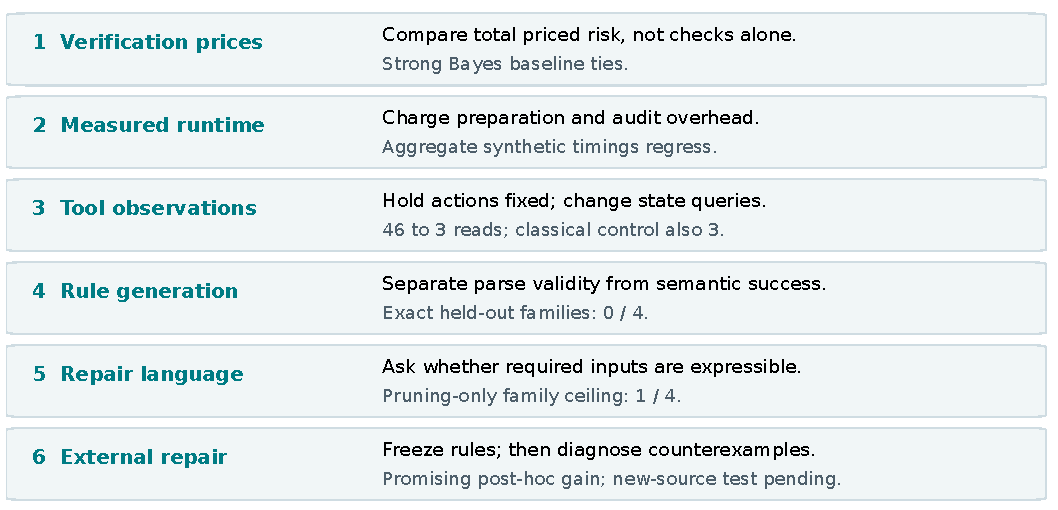
\includegraphics[width=0.98\textwidth]{pivot_map.pdf}
\caption{The pivot chain is a sequence of changed questions and controls, not a common-dataset performance trajectory. Each study preserves the earlier negative result or tie and narrows the next claim.}
\label{fig:pivots}
\end{figure*}

\section{External Evaluation: Exact Implemented Procedure}
\label{sec:externalmethod}
\subsection{Partitioning and model-pilot boundary}
A fixed label-blind normalization casefolds text, masks dates and times, UUIDs, address forms, explicit host/PID fields, hexadecimal literals, and long decimal integers, then collapses whitespace. Within each task, equal normalized strings form a group. SHA-256 parity of a fixed seed, task ID, and normalized text assigns the entire group to development or test; the first positive seed's group is forced to development. This is a structural heuristic, not campaign identity, a learned template, or the published FoRGe random split.

For the proposed six-task model pilot, eligibility required another positive development group, a positive test group, negatives in both partitions, no exact raw-string label conflict, and a description-plus-seed size limit. Twenty-three accessible tasks were eligible; a fixed hash order selected six. No prediction-dependent relaxation filled the cohort. Eligibility does not apply to every offline exploratory task, so the development metrics can have different valid denominators.

The pilot planned up to 12 local requests, with \texttt{qwen3:14b}, a fixed model digest and CPU configuration, 300-second request timeout, no paid external API, and no automatic retries. It stopped after two requests. One response has known usage of 1,209 tokens; the second request's completion and usage are unknown after timeout. The remaining ten planned requests were not run. Incomplete or unresolved predictions are not zero accuracy, a measured failure rate, or evidence that a stronger model cannot solve the task. The completed offline selectors below made no additional target-model calls.

\subsection{Finite hypothesis class and lexical extraction}
Every pattern is evaluated with \texttt{re.search} and \texttt{IGNORECASE|DOTALL}, using the reviewed upstream regex engine through a local Windows adapter. This is not reproduction of the full FoRGe harness or agent. Candidate patterns are at most 2,048 characters. Literal atoms are at most 64 characters, with at most 96 retained atoms.

The old baseline constructs atoms from one- and two-token spans of positive examples. The description-aware construction adds bounded quoted phrases and description-token atoms. Its fixed stopword list, suffix rules, substring comparison, and five-character prefix matches produce lexical features; they do not parse general negation, scope, synonymy, order, or logical intent. Description extraction retains at most 128 features, 64 quoted atoms, and 256 description atoms. An atom must match at least one supplied positive to remain eligible.

Description-aware atoms are ranked by decreasing distinct-feature coverage, increasing negative matches, decreasing positive coverage, then escaped UTF-8 length and lexical order. Retention stops at 96. Thus description information affects the class itself, not just the final choice. A phrase absent from every positive can be removed even if the description mentions it. For example, with an intended ``red or blue'' rule and only a red seed, this positive-eligibility filter can discard the blue branch. This is a structural limitation, not a newly measured corpus error.

For $n$ retained literals, the implemented grammar generates: each escaped literal; lookahead conjunction and alternation for each unordered pair of distinct literals; and an ordered \texttt{left.*right} pattern for every ordered pair, including repeats. The number generated is
\begin{equation}
n+2\binom n2+n^2=2n^2\leq18,432.
\end{equation}
The cap bounds this retained grammar, not raw-pool scanning or total runtime. Exact enumeration within this class does not optimize over all regexes. Nor does a pattern count equal the number of distinct regular languages.

\subsection{The A/B/C comparison}
All proposers accept one to three positives and zero to two negatives. Consistency means matching every supplied positive and no supplied negative. When no valid consistent candidate exists, the result is \texttt{no\_fit}; it is not silently replaced by a default-deny predictor.

\emph{A: old pool, minimum length.} The original literal baseline ranks positive-derived atoms without description coverage, retains its own pool, and selects the consistent candidate with minimum UTF-8 length, then lexical order.

\emph{B: description-aware pool, minimum length.} B uses exactly C's retained literals and generated grammar, but selects by UTF-8 length and lexical order. The worker computes it from C's returned pool, so B/C comparison holds their class fixed for the same examples.

\emph{C: description-aware pool, lexical preference.} For consistent $h$, C minimizes the lexicographic key
\begin{equation}
\bigl(-|\operatorname{cov}(h)|,\ p_{\rm OR}(h),\ |h|_{\rm UTF8},\ h\bigr).
\label{eq:selection}
\end{equation}
Coverage is the union of lexical feature sets attached to the generating literals. The alternation penalty is one when coverage is nonempty, the candidate is an alternation, and no unquoted \texttt{or/either} was found in the description. It is zero otherwise. B-to-C therefore changes coverage and this penalty jointly; it does not isolate semantic understanding. A-to-B changes pool construction and retention, so A/B/C do not all share a hypothesis class.

Two additional classical sanity baselines form an anchored escaped union of positives or use fixed variable-field masks and \texttt{SequenceMatcher}-based anti-unification. They have their own expressibility and validity limits. They are useful controls, not substitutes for strong natural-language-aware synthesis.

\subsection{Development, frozen confirmation, and post-hoc feedback}
Forty-eight tasks formed development and 17 were reserved. Before opening confirmation scores, the protocol required a candidate to run on the same 48 tasks as A and show a paired F1 increase of at least 0.05, lower FPR, nondecreasing balanced accuracy, and at least ten valid F1 pairs. Metric denominators remained explicit. C passed the recorded gate and was selected before confirmation. On development, its F1 comparison used 22 valid task pairs, FPR 45, and balanced accuracy 20; those are not 48 complete observations of each metric. B tied A on those development comparisons and was not the selected candidate.

The reserved stage froze proposals before scoring all 17 tasks once. After examining those results, a separate feedback protocol reused the same 17. It scanned each task's full development partition under the initial C rule. In source row order, the selector returns the first false positive and first false negative if both exist; otherwise it returns the first two errors of the available kind. It retains the initial seed, so the fit remains within three positives and two negatives. Five tasks had no development counterexample and retained the initial pattern for every follow-up method; twelve underwent new fits.

For each of the twelve fits, the added positives and negatives rebuild the retained pool. B and C share that rebuilt pool within the fit; it need not equal the initial pool. On the five no-feedback tasks, both follow-up policies retain initial C, rather than fitting a new B rule. The follow-up finished and hashed all proposals before evaluating the original grouped test. Test labels were not arguments to the new fitting functions. This procedural separation matters, but it cannot turn previously observed tasks into fresh confirmation. The follow-up is explicitly post hoc, not an independent replication or a new untouched holdout.

\section{External Results and Their Limits}
\label{sec:results}
\subsection{A macro improvement with poor pooled detection}
All A/B/C methods were scored on the same 17 confirmation tasks and the same 149 positive and 3,613 negative test rows. C's macro F1 was 0.5366, compared with 0.1902 for A and 0.2132 for B. Against B, C had ten task-level F1 wins, six ties, and one loss. Its mean task recall was lower, however, so the result was not Pareto dominance.

Table~\ref{tab:external} reports pooled counts alongside macro means. C yielded 100 true positives, 2,409 false positives, 1,204 true negatives, and 49 false negatives: pooled F1 0.07524, recall 0.6711, and FPR 0.6668. Reducing a very poor baseline's false positives does not establish an acceptable detector. Six tasks still flagged every negative row. Nine tasks had just one positive test row. On the other eight, C's pooled F1 was 0.08096 versus B's 0.08826; this subgroup result was a retrospective diagnostic, not a separate confirmatory hypothesis.

Macro F1 assigns equal weight to task scores; pooled F1 recomputes the ratio after summing confusion counts. Neither is inherently wrong, but they answer different finite-benchmark questions. With large differences in class counts, a claim based only on the macro improvement obscures operationally important false positives and recall losses. Neither summary estimates production performance, where prevalence and event dependencies differ.

\begin{table*}[t]
\centering\small
\setlength{\tabcolsep}{5pt}
\begin{tabular}{llrrrrrrrr}
\toprule
Stage & Method & Tasks & TP & FP & TN & FN & Macro F1 & Pooled F1 & Pooled FPR\\
\midrule
Frozen confirmation & A: old pool / length & 17 & 121 & 3,279 & 334 & 28 & 0.1902 & 0.06819 & 0.9076\\
Frozen confirmation & B: new pool / length & 17 & 121 & 3,194 & 419 & 28 & 0.2132 & 0.06986 & 0.8840\\
Frozen confirmation & C: new pool / coverage & 17 & 100 & 2,409 & 1,204 & 49 & 0.5366 & 0.07524 & 0.6668\\
\midrule
Post-hoc feedback & A: old pool / length & 15 & 45 & 473 & 2,896 & 18 & 0.5438 & 0.15491 & 0.1404\\
Post-hoc feedback & B: new pool / length & 17 & 125 & 687 & 2,926 & 24 & 0.5260 & 0.26015 & 0.1901\\
Post-hoc feedback & C: new pool / coverage & 17 & 130 & 156 & 3,457 & 19 & 0.7803 & 0.59770 & 0.0432\\
\bottomrule
\end{tabular}
\caption{Frozen confirmation and subsequent post-hoc follow-up must be interpreted separately. Confirmation A/B/C and follow-up B/C share test denominators: 149 positive and 3,613 negative rows. Follow-up A scores only 15 tasks, with 63 positive and 3,369 negative rows; its pooled values are not a common-denominator comparison to B/C. Missing/no-fit outcomes remain unresolved, not zero-error predictions. All pooled rows retain cross-task duplication.}
\label{tab:external}
\end{table*}

\begin{figure*}[t]
\centering
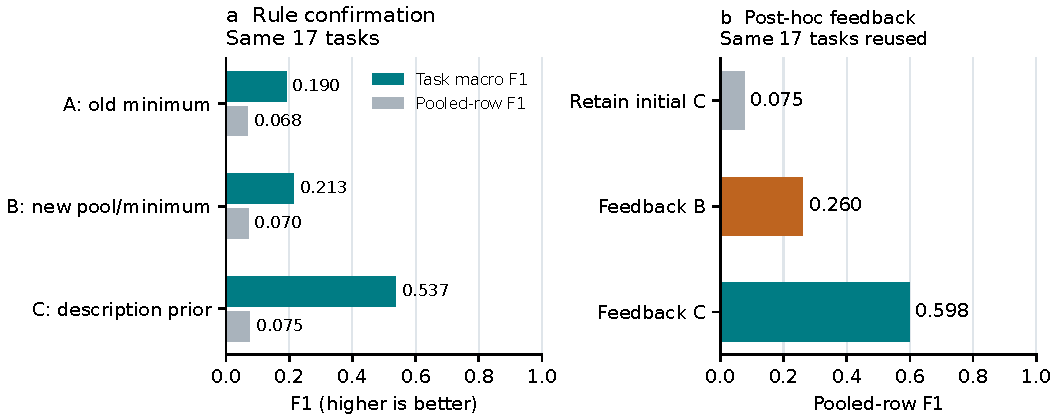
\includegraphics[width=0.96\textwidth]{external_results.pdf}
\caption{External results with distinct confirmation and post-hoc panels. Macro and pooled F1 describe different aggregations, and task counts must accompany comparisons. Feedback uses the already examined 17 tasks and supplies no independent confirmation. The main same-denominator follow-up comparison is B versus C.}
\label{fig:external}
\end{figure*}

\subsection{Counterexamples improved a post-hoc finite-benchmark result}
The follow-up compared methods using identical seed, description, and returned development feedback. C reached 130 TP, 156 FP, 3,457 TN, and 19 FN: pooled F1 0.59770, recall 0.87248, and FPR 0.04318. B reached 125 TP, 687 FP, 2,926 TN, and 24 FN: pooled F1 0.26015, recall 0.83893, and FPR 0.19015. Both have all 17 tasks, making this a properly matched finite-benchmark comparison within a shared pool. C's task-average F1 increased relative to its retained initial rule, with ten wins, five ties, and two losses.

Ten of C's 17 task outcomes were exactly correct, compared with five initially. Because five no-feedback tasks retained already exact initial results, this is five newly exact outcomes rather than ten new repairs. The results suggest that a lexical preference plus a small error-revealing example set can avoid some broad, short patterns. They do not show that this preference understands the intended rule or outperforms a strong NL-aware baseline.

Other methods have unresolved outputs: exact union scores 11/17 tasks, anti-unification 12/17, and the old literal grammar 15/17. Their valid-only denominators differ in positive and negative row counts. A high valid-only precision or low FPR cannot be ranked against a complete method while omitting no-fit or timeout outcomes. These counts remain visible in the archived scores and Appendix~\ref{app:denoms}.

The feedback mechanism compared all 4,390 development labels and returned 22 labeled counterexamples. Reporting only the 22 would conflate learner-visible information with the oracle's search cost. This is an offline simulated oracle backed by public stored labels, not a paid expert-annotation study. Human time, label validity, and the cost of discovering the right counterexamples in a real organization are unmeasured.

The follow-up used no new target-model calls. Its recorded wall time was about 227.34 seconds; known joint B/C fit CPU was 27.484375 seconds, with other known worker CPU 6.421875 seconds and two worker jobs with unknown CPU. Shared scans, fits, and cached matching make these campaign components nonadditive across methods. The initial C construction was reused, not free. These receipts describe this local execution; they do not prove a total efficiency benefit or a fair per-method deployment latency comparison.

\subsection{Dependence and unavailable comparisons}
The group split prevents within-task normalized-group overlap between development and test, but does not isolate source campaigns. Comparing all 48 development tasks with the 17 confirmation tests found 772 matching raw rows and 1,712 matching normalized rows; these overlaps were all negative. Development seed inputs had zero matching confirmation test rows. This does not prove that the fitting function received hidden test labels, but it precludes treating task IDs as independent security campaigns or using row counts as independent sample sizes.

The source's frontier-model result archives were unavailable through the release route during the original study. Those missing artifacts and the incomplete local Qwen pilot leave a direct strong-model comparison unperformed. We do not insert the original paper's published scores into our table, since the agents, available corpus, split, and evaluation differ. Likewise, we have not run Regel, SketchRegex, OpSynth, or TransRegex under the present information budget. Their absence is a substantive comparison gap.

\section{What the Pivots Explain}
\label{sec:interpretation}
The six studies separate four limitations that a single repair-success metric would hide.

\emph{Information acquisition.} In the tool experiment, unknown membership mattered only when admissible hidden values led to different actions. In the feedback study, a short returned message depended on a full labeled development scan. Query count alone did not measure the resource needed to obtain useful information.

\emph{Representation.} The policy diagnostic showed a hard boundary for a specified repair class: no amount of better ranking can add a field that every candidate ignores. In the regex experiment, a bounded literal class also excludes many meaningful patterns. Increasing test accuracy within the class does not imply the class represents the desired language.

\emph{Selection.} Where the reference is expressible, selectors can still choose poorly. Minimal syntactic length may select a broad generic token; a lexical score may overfit incidental words, misread explicit disjunction, or prefer an ordered gap for an order-independent description. B/C isolates a particular selector change within one retained class; it does not establish a generally optimal semantic prior.

\emph{Evaluation.} A virtual price is not time, one source method is not a full service episode, an authored context is not an independent policy, and a macro gain is not a practical false-alarm rate. A post-hoc improvement on previously observed tests may motivate a hypothesis, but it cannot confirm that hypothesis on fresh data.

These distinctions also explain why different negative results call for different pivots. A tie with strong Bayes asks whether the proposed stopping method adds anything. Aggregate timing regression asks whether overhead and reference quality were realistic. A representation ceiling asks whether more queries can matter at all. Poor pooled external detection asks whether a favorable metric matches the application. None is repaired by merely increasing the number of branches, candidates, or presentation artifacts.

\section{Related Work and Contribution Boundary}
Natural-language-to-regex synthesis predates this project. Kushman and Barzilay use semantic unification to address variation among equivalent regex representations \cite{kushman2013}. Regel translates descriptions to hierarchical sketches that guide example-based synthesis \cite{regel2020}. SketchRegex also combines incomplete sketches and consistency with examples \cite{sketchregex2020}. TransRegex explicitly combines generation with example-driven repair \cite{transregex2021}. These establish that the broad modalities and repair structure are existing approaches; their reported performance is not reproduced here.

OpSynth is especially close to the abstract selection objective: satisfy behavioral examples while maximizing a natural-language-conditioned model score \cite{opsynth2021}. Our archived C selector replaces a learned score with a fixed lexical coverage key and enumerates a small retained class. That is an implementation and empirical-scope distinction, not evidence of a novel general synthesis principle. FoRGe already provides the single-example log-rule problem and an agent that explores log data using feedback \cite{forge2026}. Our no-unlabeled-pool deterministic setting uses different information and cannot serve as a reproduction of that full system.

The contribution claimed here is therefore an explicit reconstruction of a particular empirical program: the controls that eliminated broad claims, the representation diagnostic explaining a restricted success ceiling, and the contrast between frozen confirmation and a promising but post-hoc feedback result. The six primary external works were selected for direct overlap; this is not a systematic literature review or a proof that no other relevant work exists. Reproducible archival consistency supports the reconstruction, not novelty certification or scientific acceptance.

\section{A Falsifiable Next Study}
\label{sec:future}
The next question is whether feedback benefit remains against stronger information-matched baselines on new sources after accounting for the acquisition process and missed detections. This section states a proposed design; none of its outcomes is asserted as observed.

Before accessing new evaluation labels, freeze the exact class construction, all caps, flags, feedback selection, failure handling, metrics, cost boundaries, and stopping rules. New source groups must be separated by actual provenance where possible, with source dependence disclosed when provenance is insufficient. The current 17 tasks remain development evidence for this purpose and cannot serve as a new untouched confirmation cohort.

Include a simple description-aware keyword/conjunction rule as well as at least one reproducible close synthesis baseline under the same available information. The existing length-only B ablation is useful but not the strongest plausible competitor. A method that wins only because its baseline ignores description content does not establish an advantage in integrating natural language.

Pair each seed with the original description, a meaning-preserving paraphrase, a removed description, and an unrelated description, fixed without outcome feedback. Negation, order, and alternative-branch conditions should be predefined stress strata. Repeated descriptions of one task remain repeated measurements, not independent tasks. These controls can distinguish useful description information from generic changes in rule length or pool retention.

Report task-level and source-level counts, raw TP/FP/TN/FN, macro and pooled metrics, no-fit, invalid, timeout, unexecuted outcomes, and common-denominator paired comparisons. Fix application-relevant false-positive and missed-detection requirements before claiming practical success. Do not infer precise population significance from many dependent log rows; choose an uncertainty analysis appropriate to the actual source units and available sample.

Separate representation from selection by evaluating a post-hoc oracle upper bound within a frozen class only as a diagnostic. A label-selected oracle is not an executable baseline. Count all feedback search, adjudication, labeling, preparation, generation, enumeration, verification, and failed requests. Where human cost or usage remains unknown, retain that gap rather than claiming savings. If the effect vanishes against stronger NL-aware baselines or new sources, preserve that negative result and abandon the algorithm-superiority interpretation.

\section{Limitations and Research Integrity}
The earlier studies are small, heterogeneous, and mostly in-house. Public code verdicts can inherit evaluator errors; controlled byte timing on one PC does not generalize to model-serving or storage workloads; policy labels encode authored interpretations; and the external logs are simulation-derived and not independently reannotated here. The blocked external file leaves the full corpus incomplete. No result certifies a safe detector or a valid complete customer-service policy.

The chronology imposes additional limits. The overall 880-verdict class counts were known, the external leader had seen development outcomes, and the feedback follow-up reused examined confirmation tasks. No p-values, confidence claims for dependent task populations, or global novelty claims are supplied. The finite projection argument and exhaustive selectors are applications of elementary reasoning, not new theoretical results.

Local regex execution used subprocess timeouts and bounded pattern lengths. A timeout limits a process duration but is not an OS security sandbox. External log strings and model outputs were treated as data. The study made no production-security deployment, actual payment, external submission, or operational promotion. Existing source records and unresolved calls were preserved.

AI systems assisted code, diagnostic patches, literature review, analysis, and manuscript preparation. AI-authored evaluation and independent AI recalculation are not independent human expert validation. The manuscript does not infer an unstated model version for drafting or claim that author confirmation has occurred. Source-policy interpretation, external label validity, and publication declarations require further author and specialist review.

\section{Conclusion}
The ProbeFlow record supports a methodological pivot from broad repeated-repair claims toward a costed, representation-aware empirical question. Conditional virtual savings tied a strong classic baseline; measured timing did not show general speedup; fewer tool reads tied explicit classical reasoning; and policy-repair failure partly reflected a repair language that could not express the missing conditions. On external logs, a favorable macro score concealed poor pooled detection. Counterexamples then improved a fixed lexical selector on the same previously observed tasks, while full-pool label scans and unresolved outcomes bounded the interpretation.

The defensible result is the documented sequence of these constraints and a concrete follow-up hypothesis. Establishing a new method or a practical advantage still requires new source groups, stronger information-matched comparators, label validation, and measured acquisition and failure costs. The present draft preserves those open requirements.

\section*{Acknowledgements}
This work was created as part of the No-More-Slops group activities at Pseudo Lab.

\begingroup
\small
\bibliographystyle{plain}
\bibliography{references}
\endgroup

\appendix
\section{Evidence Map and Reproducibility Boundary}
\label{app:evidence}
All local paths below are relative to the repository's \archive{outputs/} directory. They identify the scientific archives, not an assertion that a public repository contains the data. The delivery source manifest binds exact files and hashes. Long names are broken across lines for readability.

\begin{description}
\item[P1] \archive{probeflow_paid_verification_20261116_01}: \archive{design/PROTOCOL_KO.txt}, \archive{results/SUMMARY.json}, \archive{records/CANDIDATE_DECISION.json}, and the archived independent-replay receipt.
\item[P2] \archive{probeflow_measured_audit_20261116_01}: \archive{records/CANDIDATE_DECISION.json}, frozen design, summary, robustness diagnostic, and independent-replay records.
\item[P3] \archive{probeflow_evidence_compiler_20261119_01}: \archive{records/RESEARCH_DECISION_KO.txt} and linked identifiability, provenance, and heuristic-diagnostic records.
\item[P4] \archive{probeflow_contract_learning_20261119_01}: \archive{records/RESEARCH_DECISION_KO.txt}, \archive{records/BUNDLE_BINDING.json}, and the frozen generation/evaluation records.
\item[P5] \archive{probeflow_repair_identifiability_20261120_01}: \archive{records/RESEARCH_DECISION_KO.txt}, \archive{records/BUNDLE_BINDING.json}, and the linked lower-bound, query, and constructive-patch diagnostics.
\item[P6] \archive{probeflow_external_validation_20261120_01}: original protocol and amendment; \archive{records/CORPUS_AUDIT.json}; \archive{implementation/classical.py}, \archive{description_prior.py}, \archive{prior_worker.py}, \archive{pilot.py}, \archive{feedback_probe.py}; \archive{records/PRIOR_PROTOCOL_KO.txt}; \archive{records/DEVELOPMENT_DECISION.json}; \archive{validation_prior_01/SUMMARY.json}; \archive{records/CONFIRMATION_AUDIT.json}; \archive{records/CROSS_COHORT.json}; \archive{records/FEEDBACK_PROBE_PROTOCOL_KO.txt}; \archive{feedback_probe_01/SUMMARY.json}; and associated frozen proposal and test-score receipts.
\end{description}

The external implementation's frozen classical SHA-256 is \texttt{cdc527011fccc24be023c31eb4c129e06}\allowbreak\texttt{c183f23a5be34f2bc7035fee3b663e6}; description-prior SHA-256 is \texttt{b668a9ab80fabdaf4dd8e66e9842ffa590}\allowbreak\texttt{b689b68cfc832fe3ad474c14a88f20}. The prior module checks its grammar dependency before use. Confirmation proposals were frozen at SHA-256 \texttt{7c65c3ec6684bb267c674874d42760926a}\allowbreak\texttt{a2cef286063bacf64a4d3c686fe98a}. These fingerprints establish which local files were evaluated, subject to the recorded source-access boundary; they do not certify labels, scientific conclusions, or model-weight equivalence.

The source's \archive{powershell_webrequest_using_memory_stream.json} remained inaccessible. This paper does not require reading it. Reproduction must preserve the scope amendment and report 65 accessible tasks rather than silently treating the declared 66 as reverified. The full upstream source harness, frontier-model archives, and downloaded code were not executed as part of this manuscript preparation.

\section{Denominators, Failures, and Shared Costs}
\label{app:denoms}
\begin{table}[h]
\centering\small
\setlength{\tabcolsep}{3pt}
\begin{tabular}{p{0.44\columnwidth}rrr}
\toprule
Post-hoc method & Tasks & Pos. & Neg.\\
\midrule
Retained initial C & 17/17 & 149 & 3,613\\
Exact union & 11/17 & 50 & 2,816\\
Anti-unification & 12/17 & 54 & 2,948\\
Old literal grammar A & 15/17 & 63 & 3,369\\
Shared-pool length B & 17/17 & 149 & 3,613\\
Description preference C & 17/17 & 149 & 3,613\\
\bottomrule
\end{tabular}
\caption{Valid-only denominators in the feedback follow-up. Tasks denotes scored/attempted tasks; Pos. and Neg. count their positive and negative rows. Different denominators prevent interpreting every pooled score as a matched comparison.}
\end{table}

The original external Qwen pilot's incomplete status is separate from these deterministic experiments. It selected six tasks and planned up to 12 calls, but made two attempts. One initial response reported 1,209 tokens; a later request exceeded the 300-second client limit and has unknown completion and usage. Ten planned calls remained unexecuted. A stored null metric means unresolved or unobserved, not an observed zero. The record does not permit estimating complete-model accuracy or total token expenditure by filling those gaps.

In the deterministic confirmation, A/B/C all produced scored outputs for 17 tasks. Recorded joint fit CPU was 16.4375 seconds and matching CPU 0.265625 seconds; total recorded wall was about 58.00 seconds. This joint execution computed both B and C and reused earlier A artifacts. It is not C's independent deployment cost. In the feedback follow-up, all 17 development partitions were scanned, comparing 4,390 labels and returning 22. Twelve new joint B/C fits were run; five no-feedback cases retained initial patterns. Pattern matching was cached where methods returned identical patterns. The same scan cannot be added once per method and then called actual spending.

Reported local CPU components exclude unknown worker CPU and do not measure human effort, research-assistant inference, data adjudication, or electricity. Earlier initial-model cost also persists when a later stage uses zero new target-model calls. The complete research cost remains unmeasured in every scientific archive considered here.

\end{document}
